\section{MLOps}\label{sec:mlops}

In this section we will try to describe key aspect of MLOps as can be found in today's literature.

\subsection{Description}\label{subsec:description}
MLOps or Machine Learning Operations is the automation of Machine learning development workflow and operations.
It's an extension of DevOps practices adapted to machine learning model development and data operations.
MLOps almost never taken alone and DataOps is an integrated part of the full MLOps lifecycle.

\begin{figure}[!htbp]
    \caption{MLOps lifecycle \cite{mlops-definition-tools-and-challenge}}
    \centering
    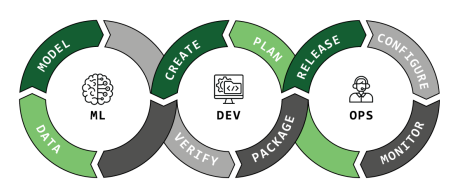
\includegraphics[scale=0.5]{images/ml-dev-ops}
    \label{fig:ml-dev-ops}
\end{figure}

\subsection{Maturity Models}\label{subsec:maturity-models}
\cite{mlops-maturity-model} they propose a maturity model that goes from manual MLOps to fully automated MLOps.
It differs from the Microsoft and the Google MLOps maturity models,
but they all tend to go from manual to fully automated MLOps processes using automated CI/CD and
ML pipelines.\cite{mlops-definition-tools-and-challenge}

\begin{figure}[!htbp]
    \caption{Maturity levels \cite{mlops-maturity-model}}
    \centering
    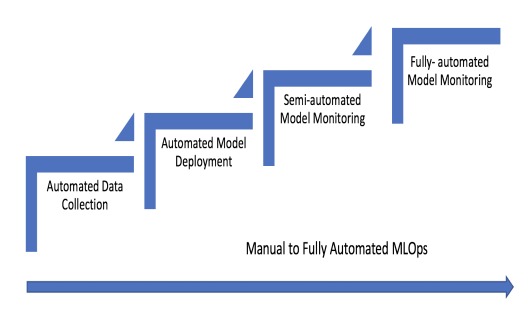
\includegraphics[scale=0.5]{images/maturity-levels}
    \label{fig:maturity}
\end{figure}

\subsection{MLOps Workflow}\label{subsec:mlops-workflow}